\documentclass[10pt,twocolumn,letterpaper]{article}

\usepackage{cvpr}
\usepackage{times}
\usepackage{epsfig}
\usepackage{graphicx}
\usepackage{amsmath}
\usepackage{amssymb}
\usepackage[utf8]{inputenc}
\usepackage{fullpage}
\usepackage{subfig}

\usepackage[margin=1in]{geometry} 
\usepackage{amsmath,amsthm,amssymb}
 
\newcommand{\N}{\mathbb{N}}
\newcommand{\Z}{\mathbb{Z}}
 
\newenvironment{theorem}[2][Theorem]{\begin{trivlist}
\item[\hskip \labelsep {\bfseries #1}\hskip \labelsep {\bfseries #2.}]}{\end{trivlist}}
\newenvironment{lemma}[2][Lemma]{\begin{trivlist}
\item[\hskip \labelsep {\bfseries #1}\hskip \labelsep {\bfseries #2.}]}{\end{trivlist}}
\newenvironment{exercise}[2][Exercise]{\begin{trivlist}
\item[\hskip \labelsep {\bfseries #1}\hskip \labelsep {\bfseries #2.}]}{\end{trivlist}}
\newenvironment{reflection}[2][Reflection]{\begin{trivlist}
\item[\hskip \labelsep {\bfseries #1}\hskip \labelsep {\bfseries #2.}]}{\end{trivlist}}
\newenvironment{proposition}[2][Proposition]{\begin{trivlist}
\item[\hskip \labelsep {\bfseries #1}\hskip \labelsep {\bfseries #2.}]}{\end{trivlist}}
\newenvironment{corollary}[2][Corollary]{\begin{trivlist}
\item[\hskip \labelsep {\bfseries #1}\hskip \labelsep {\bfseries #2.}]}{\end{trivlist}}
 


% Include other packages here, before hyperref.

% If you comment hyperref and then uncomment it, you should delete
% egpaper.aux before re-running latex.  (Or just hit 'q' on the first latex
% run, let it finish, and you should be clear).
\usepackage[breaklinks=true,bookmarks=false]{hyperref}

\cvprfinalcopy % *** Uncomment this line for the final submission

\def\cvprPaperID{****} % *** Enter the CVPR Paper ID here
\def\httilde{\mbox{\tt\raisebox{-.5ex}{\symbol{126}}}}

% Pages are numbered in submission mode, and unnumbered in camera-ready
%\ifcvprfinal\pagestyle{empty}\fi
\setcounter{page}{1}
\begin{document}

%%%%%%%%% TITLE
\title{Clasificadores PHOW}

\author{Francisco J. Cedano\\
Departamento de Ingenier\'ia Biom\'edica\\
Universidad de Los Andes\\
{\tt\small fj.cedano803@uniandes.edu.co}
% For a paper whose authors are all at the same institution,
% omit the following lines up until the closing ``}''.
% Additional authors and addresses can be added with ``\and'',
% just like the second author.
% To save space, use either the email address or home page, not both
}%\and
%Second Author\\
%Institution2\\
%First line of institution2 address\\
%{\tt\small secondauthor@i2.org}


\maketitle
%\thispagestyle{empty}

%%%%%%%%% ABSTRACT
\begin{abstract}
   En el presente laboratorio se estudian métodos para reconocimiento imágenes en categorías respectivas usando la base de datos caltech101 y la base de datos imagenet-tiny, esta segunda contiene imágenes de mayor complejidad. Los métodos usados se basan en PHOW (descriptores SIFT multi-escala. En este trabajo se variaron diferentes variables en el método, con el fin de estimar la exactitud de los métodos y el costo computacional.
   
\end{abstract}

%%%%%%%%% BODY TEXT
\section{Introducción}

Se usaron dos diferentes bases de datos en este proyecto. La primera es caltech101 (ver Figura 1.) la cual contiene 101 clases de objetos, tales como: elefantes, computadores personaels, ventiladores, etc. Son cerca de 40 a 800 imágenes por categoría. La mayoría tiene cerca de 50 imágenes. El tamaño de cada imágen es de aproximadametne 300x200 píxeles. Por otro lado, la base de datos de imagenet-tiny, tiene 

\begin{figure}[ht]
\centering
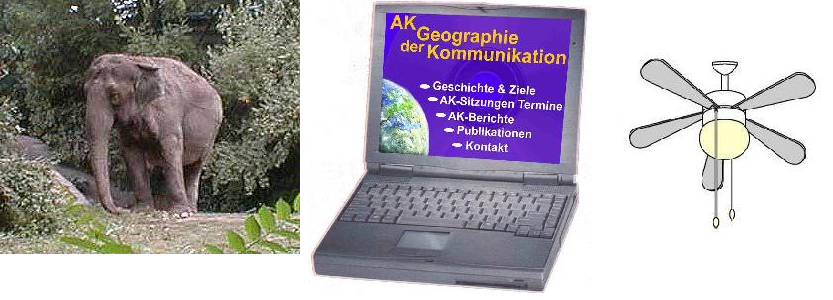
\includegraphics[width=1\linewidth]{caltech.png}
\caption{Ejemplos de imágenes de la base de datos Caltech101. (izq.) Imagen de la clase elephant, (ctro) Imagen de la clase Laptops y (der.) Imagen de la clase celling\_fan}
\end{figure}

\begin{figure}[ht]
\centering
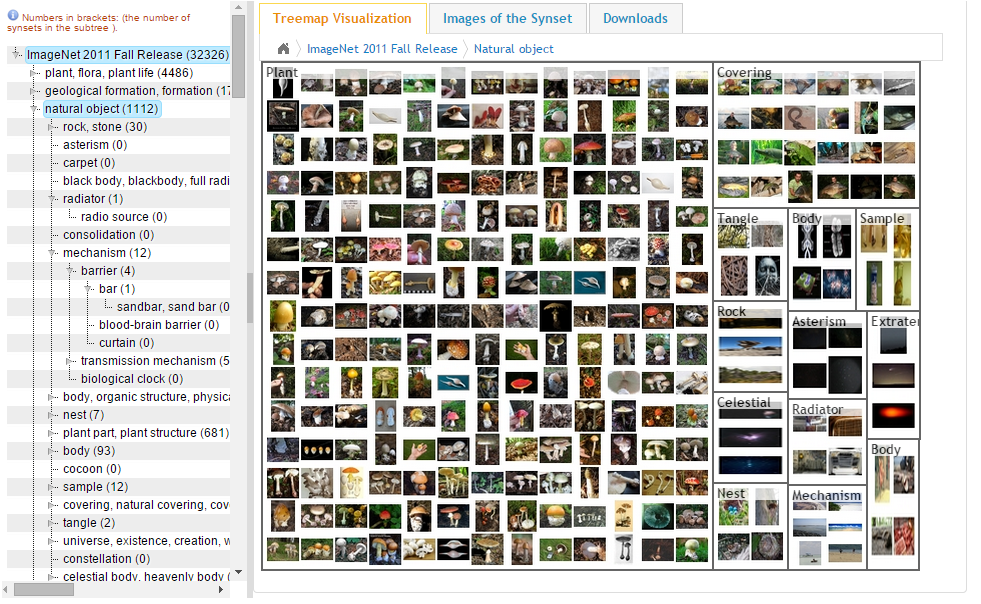
\includegraphics[width=1\linewidth]{BaseDatos.png}
\caption{Ejemplo de asignación de textones en una imagen de la categoría brick1, (izq.) Imagen original y (der.) mapa de textones.}
\end{figure}



%------------------------------------------------------------------------
\section{Metodología}




\begin{figure}[ht]
\centering

 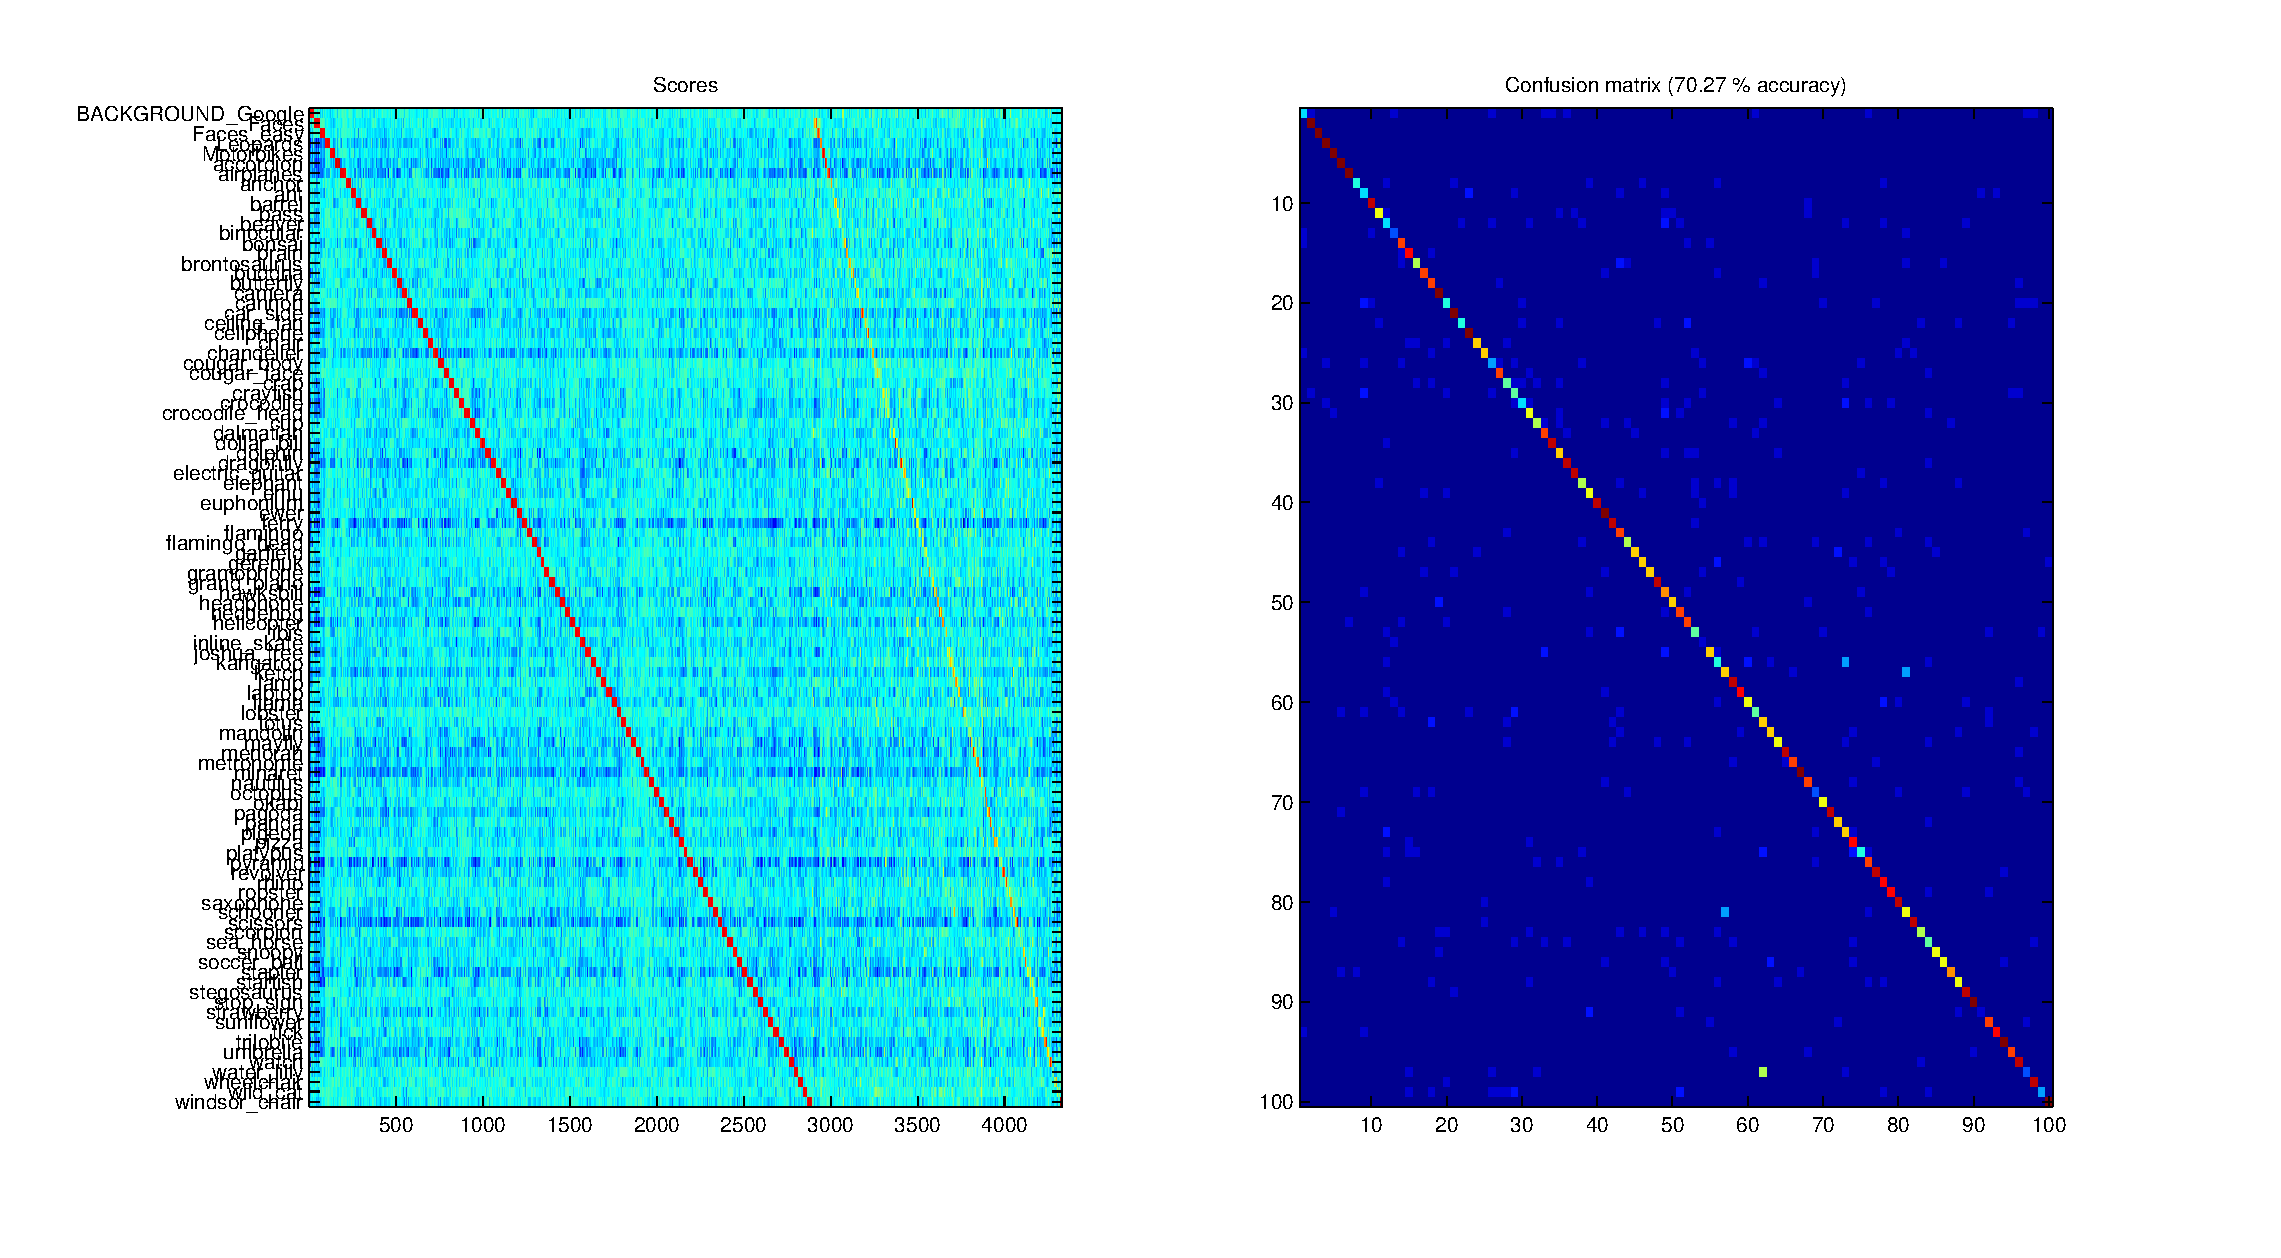
\includegraphics[width=1\linewidth]{Ejemplo_Res_Cal.eps}

\end{figure}


\subsection{Clasificadores}

\subsection{Resultados}
\begin{figure}[ht]
\centering

 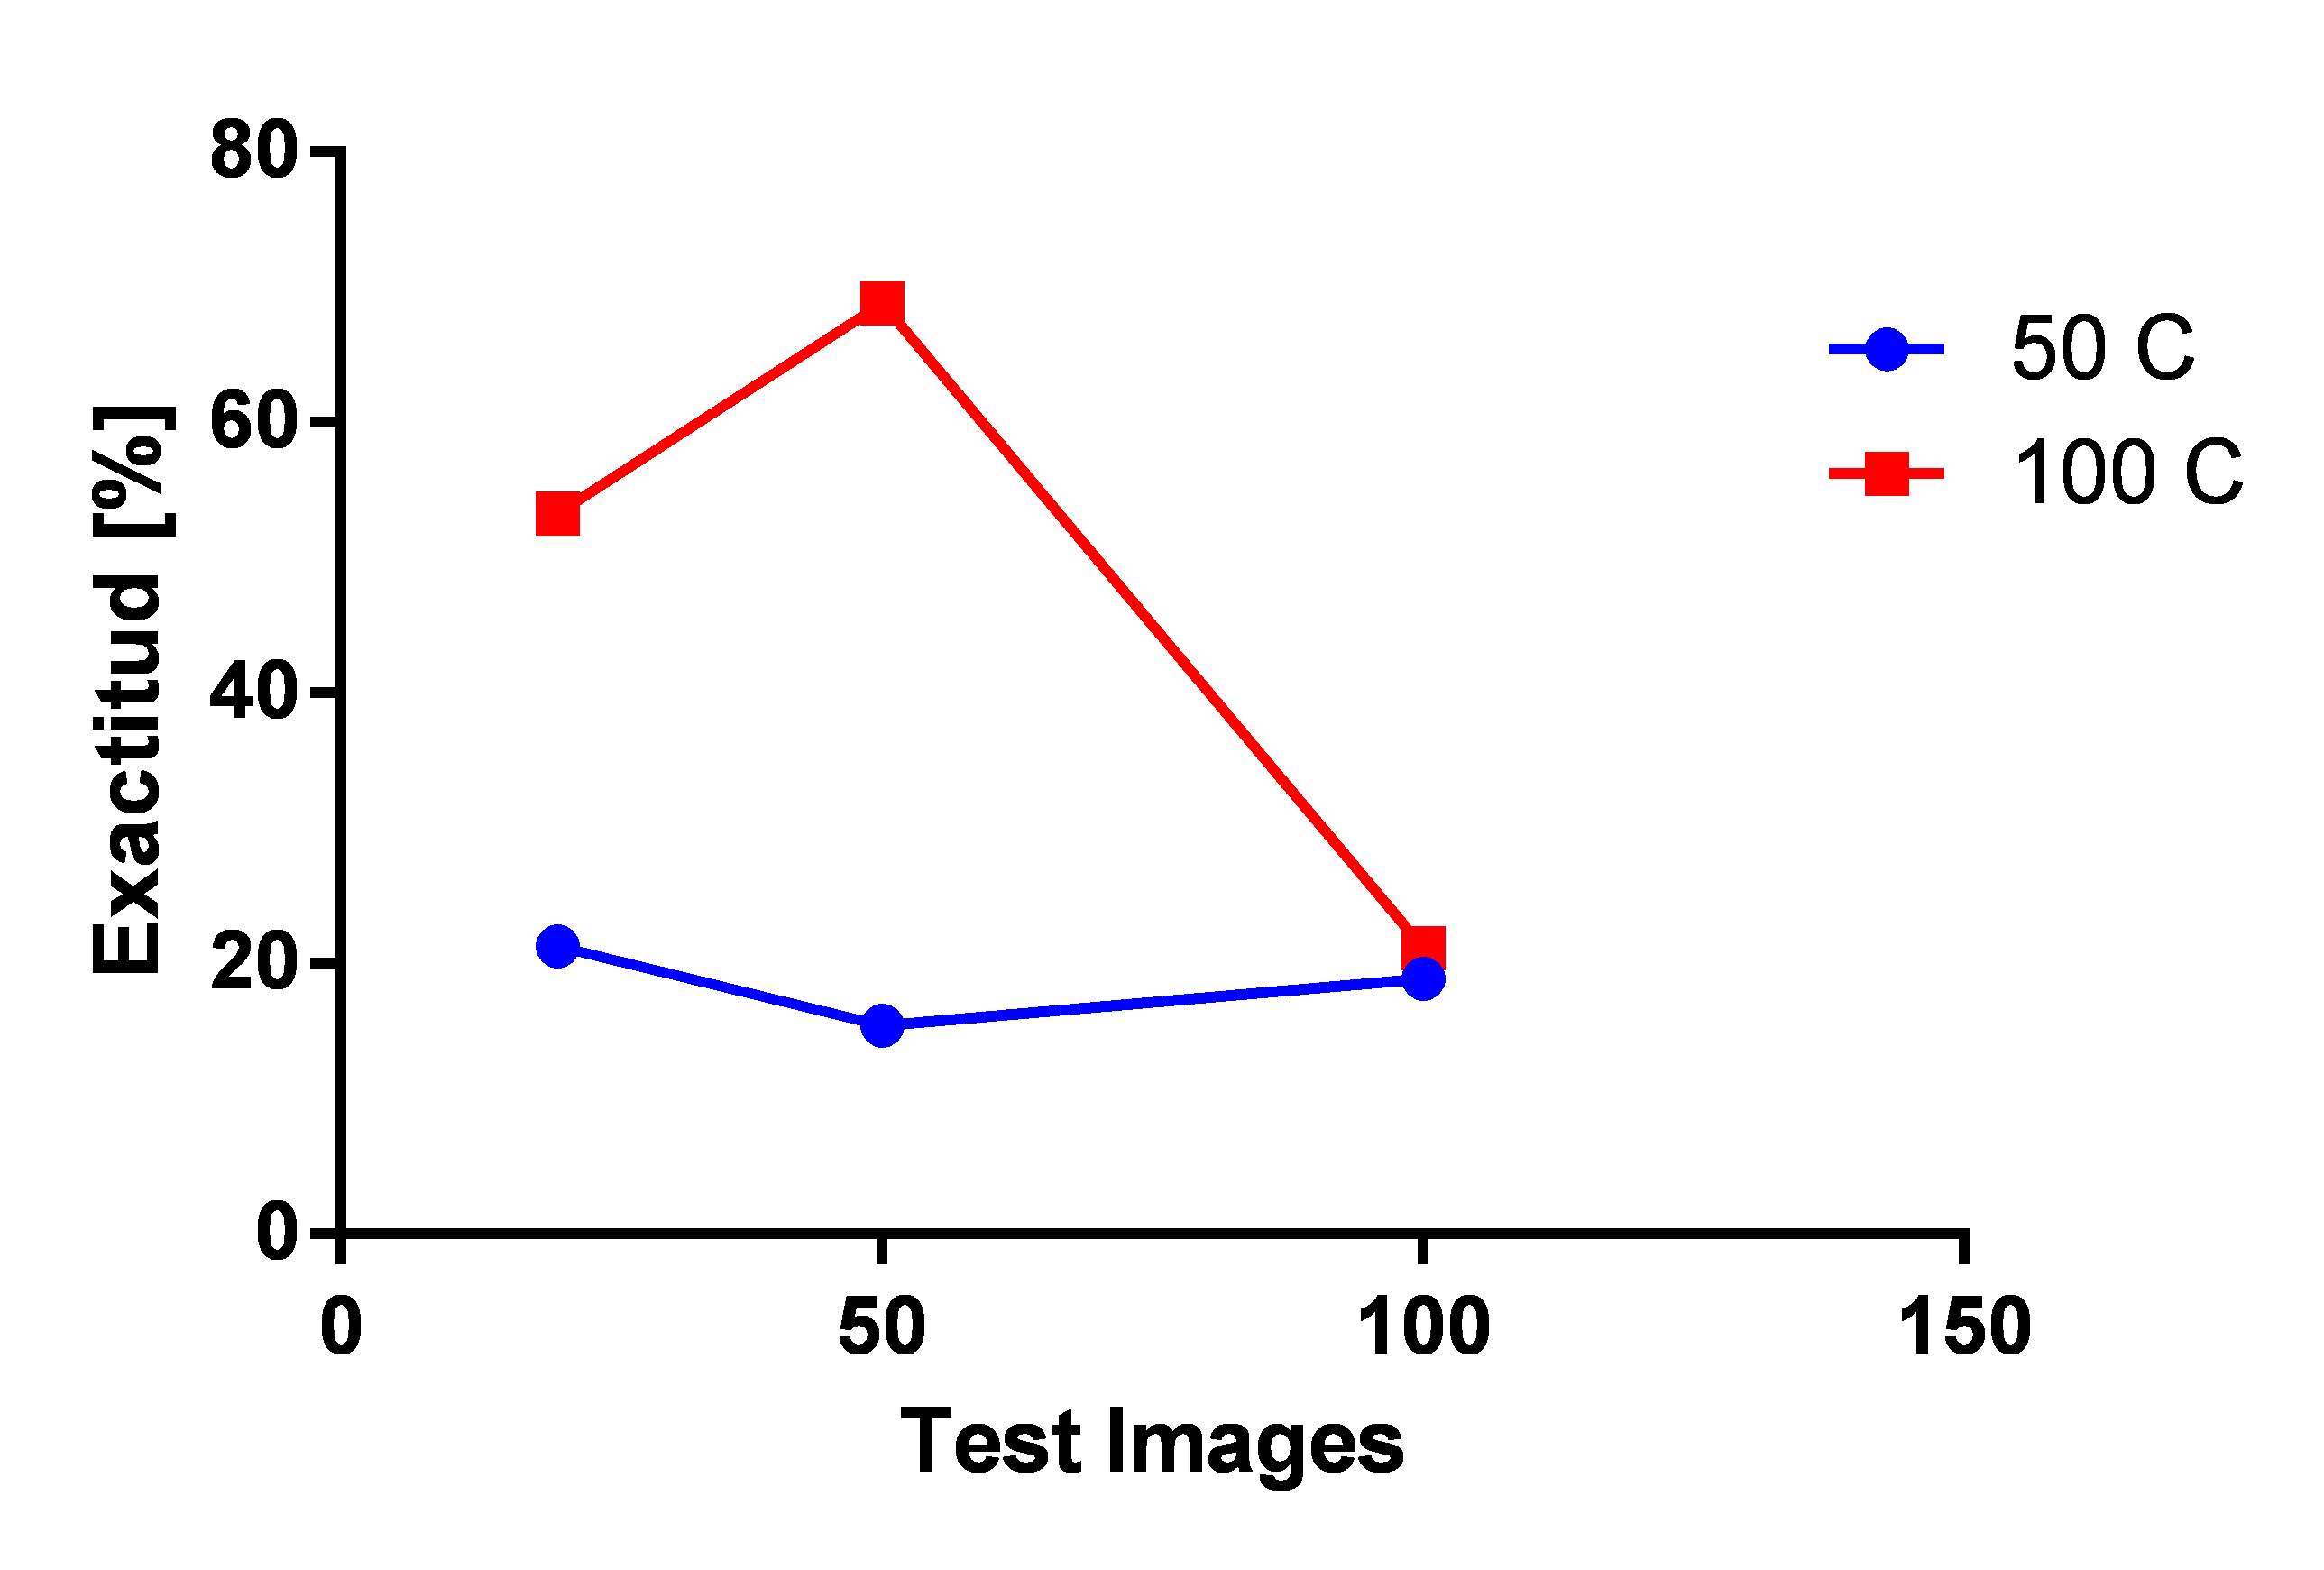
\includegraphics[width=1\linewidth]{Test_images.png}

\end{figure}


\begin{figure}[ht]
\centering

 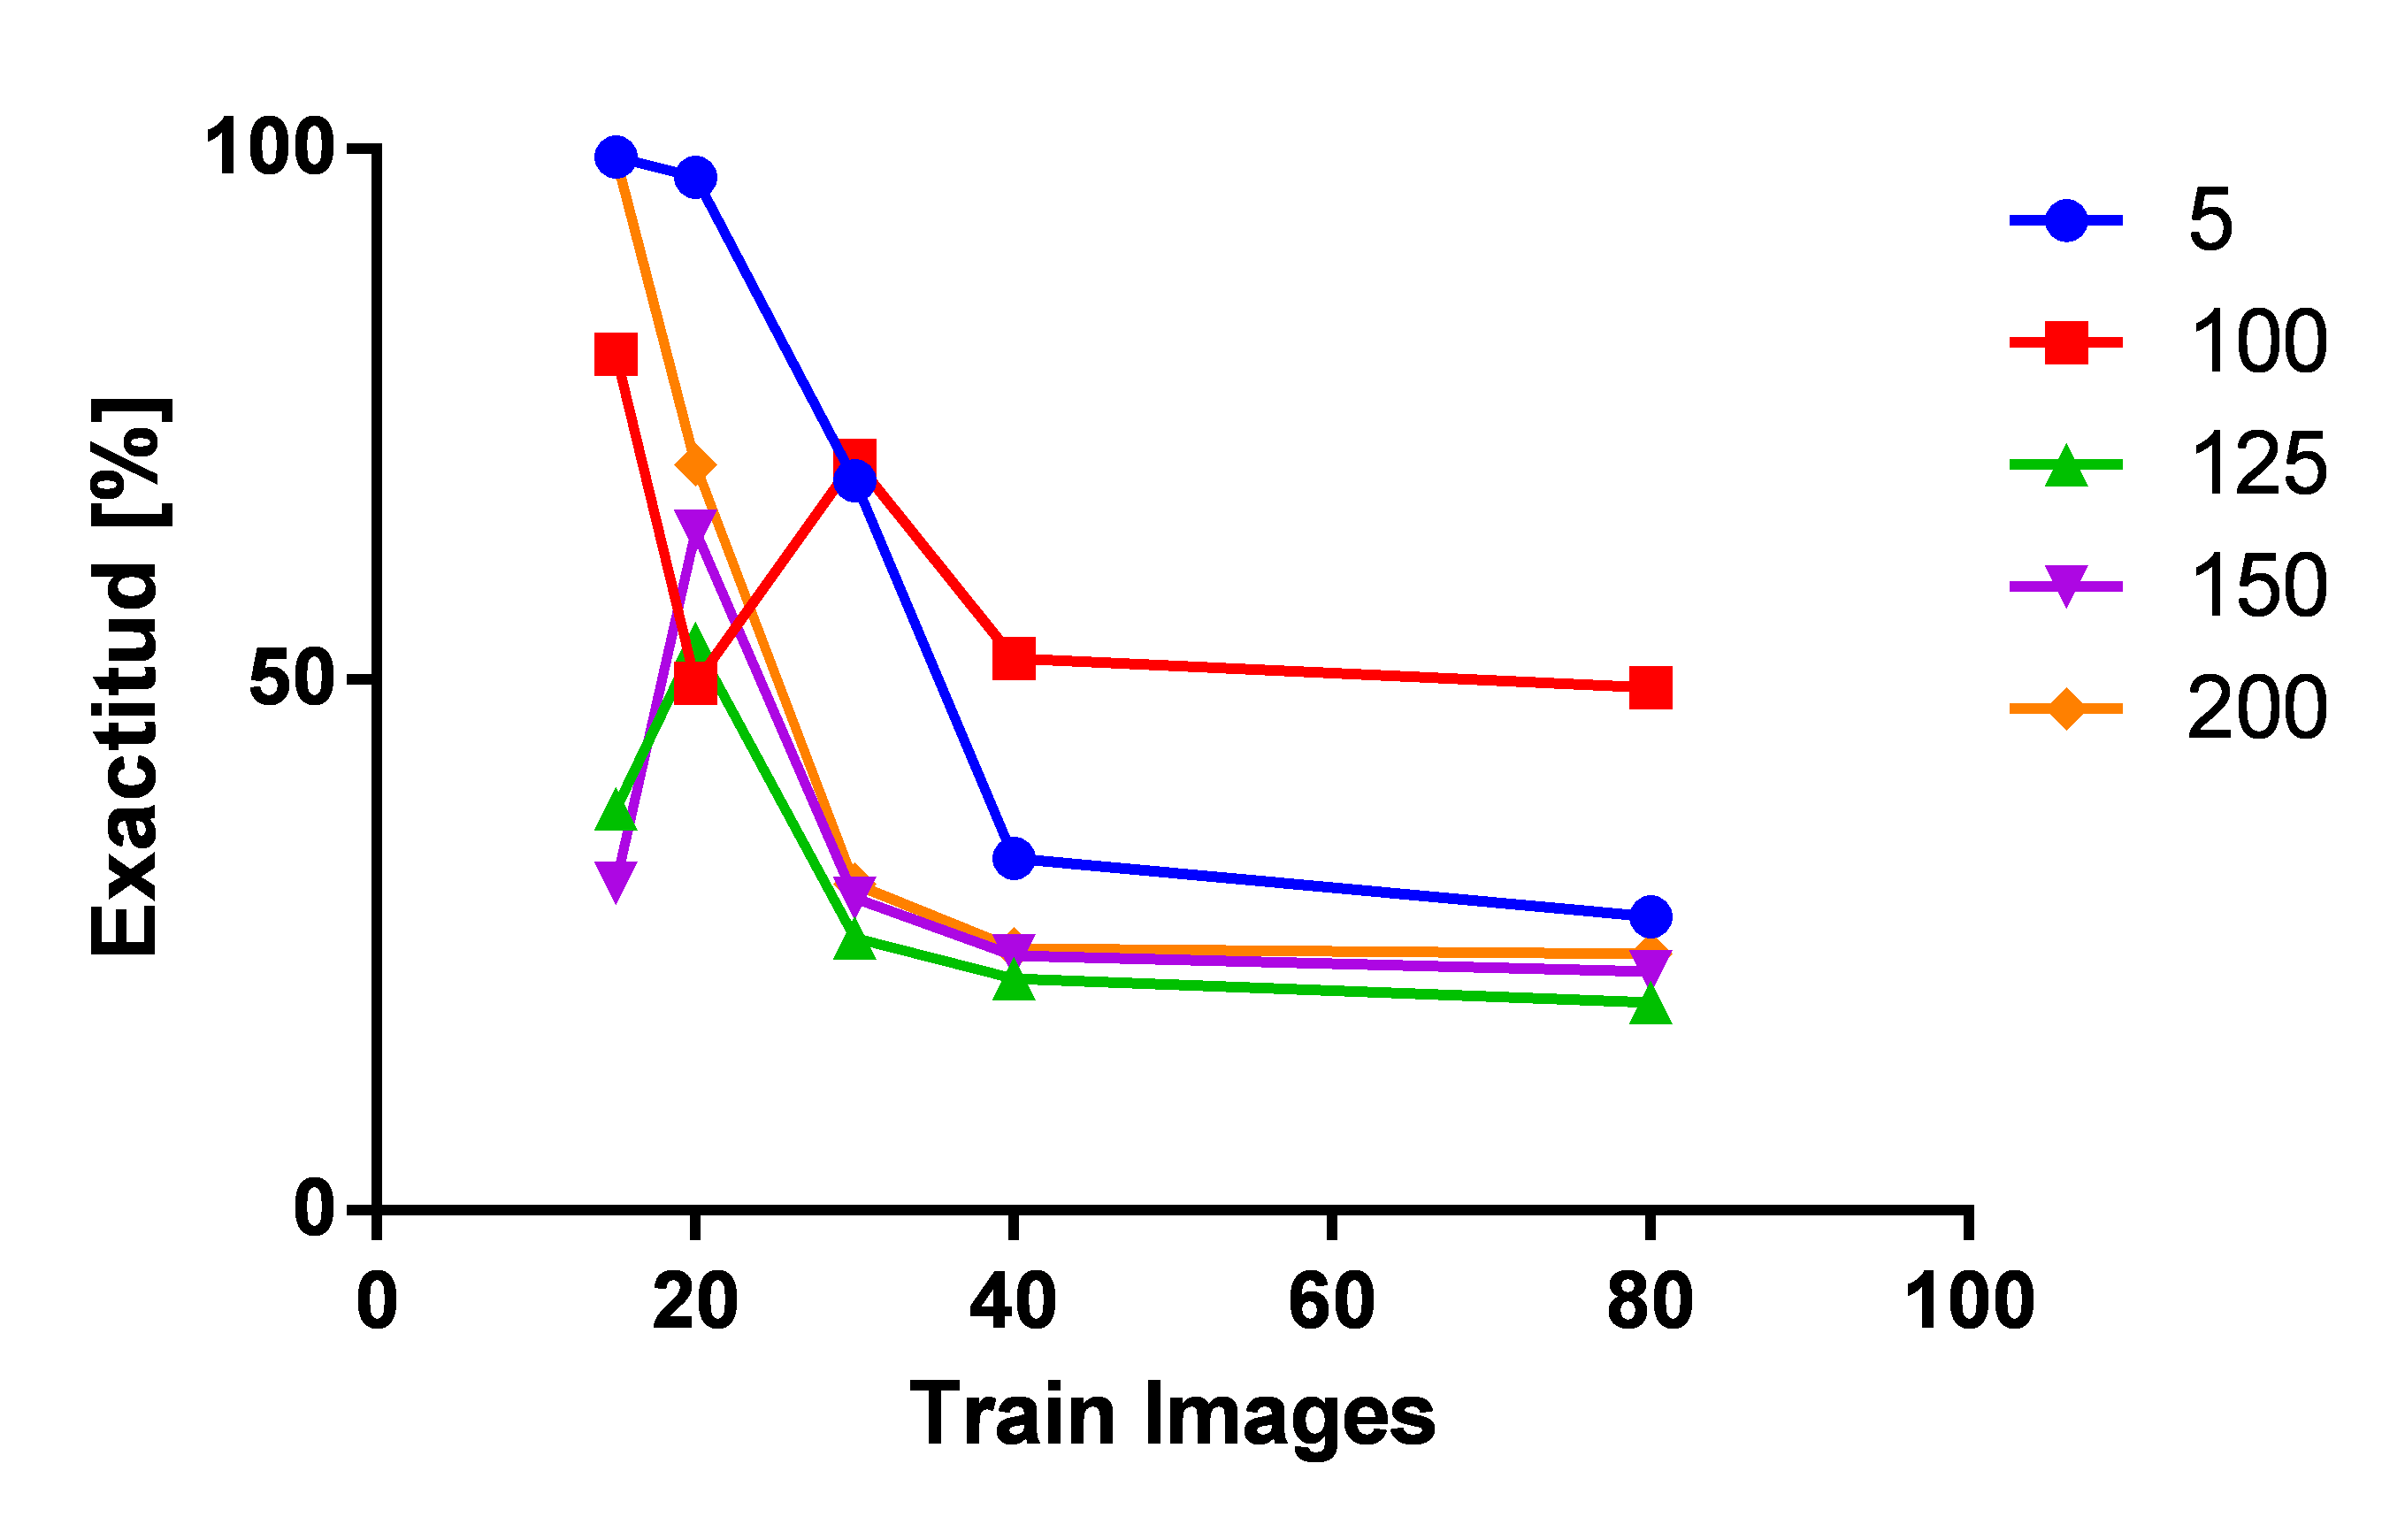
\includegraphics[width=1\linewidth]{Resutlado_Train.png}

\end{figure}

\begin{figure}[ht]
\centering

 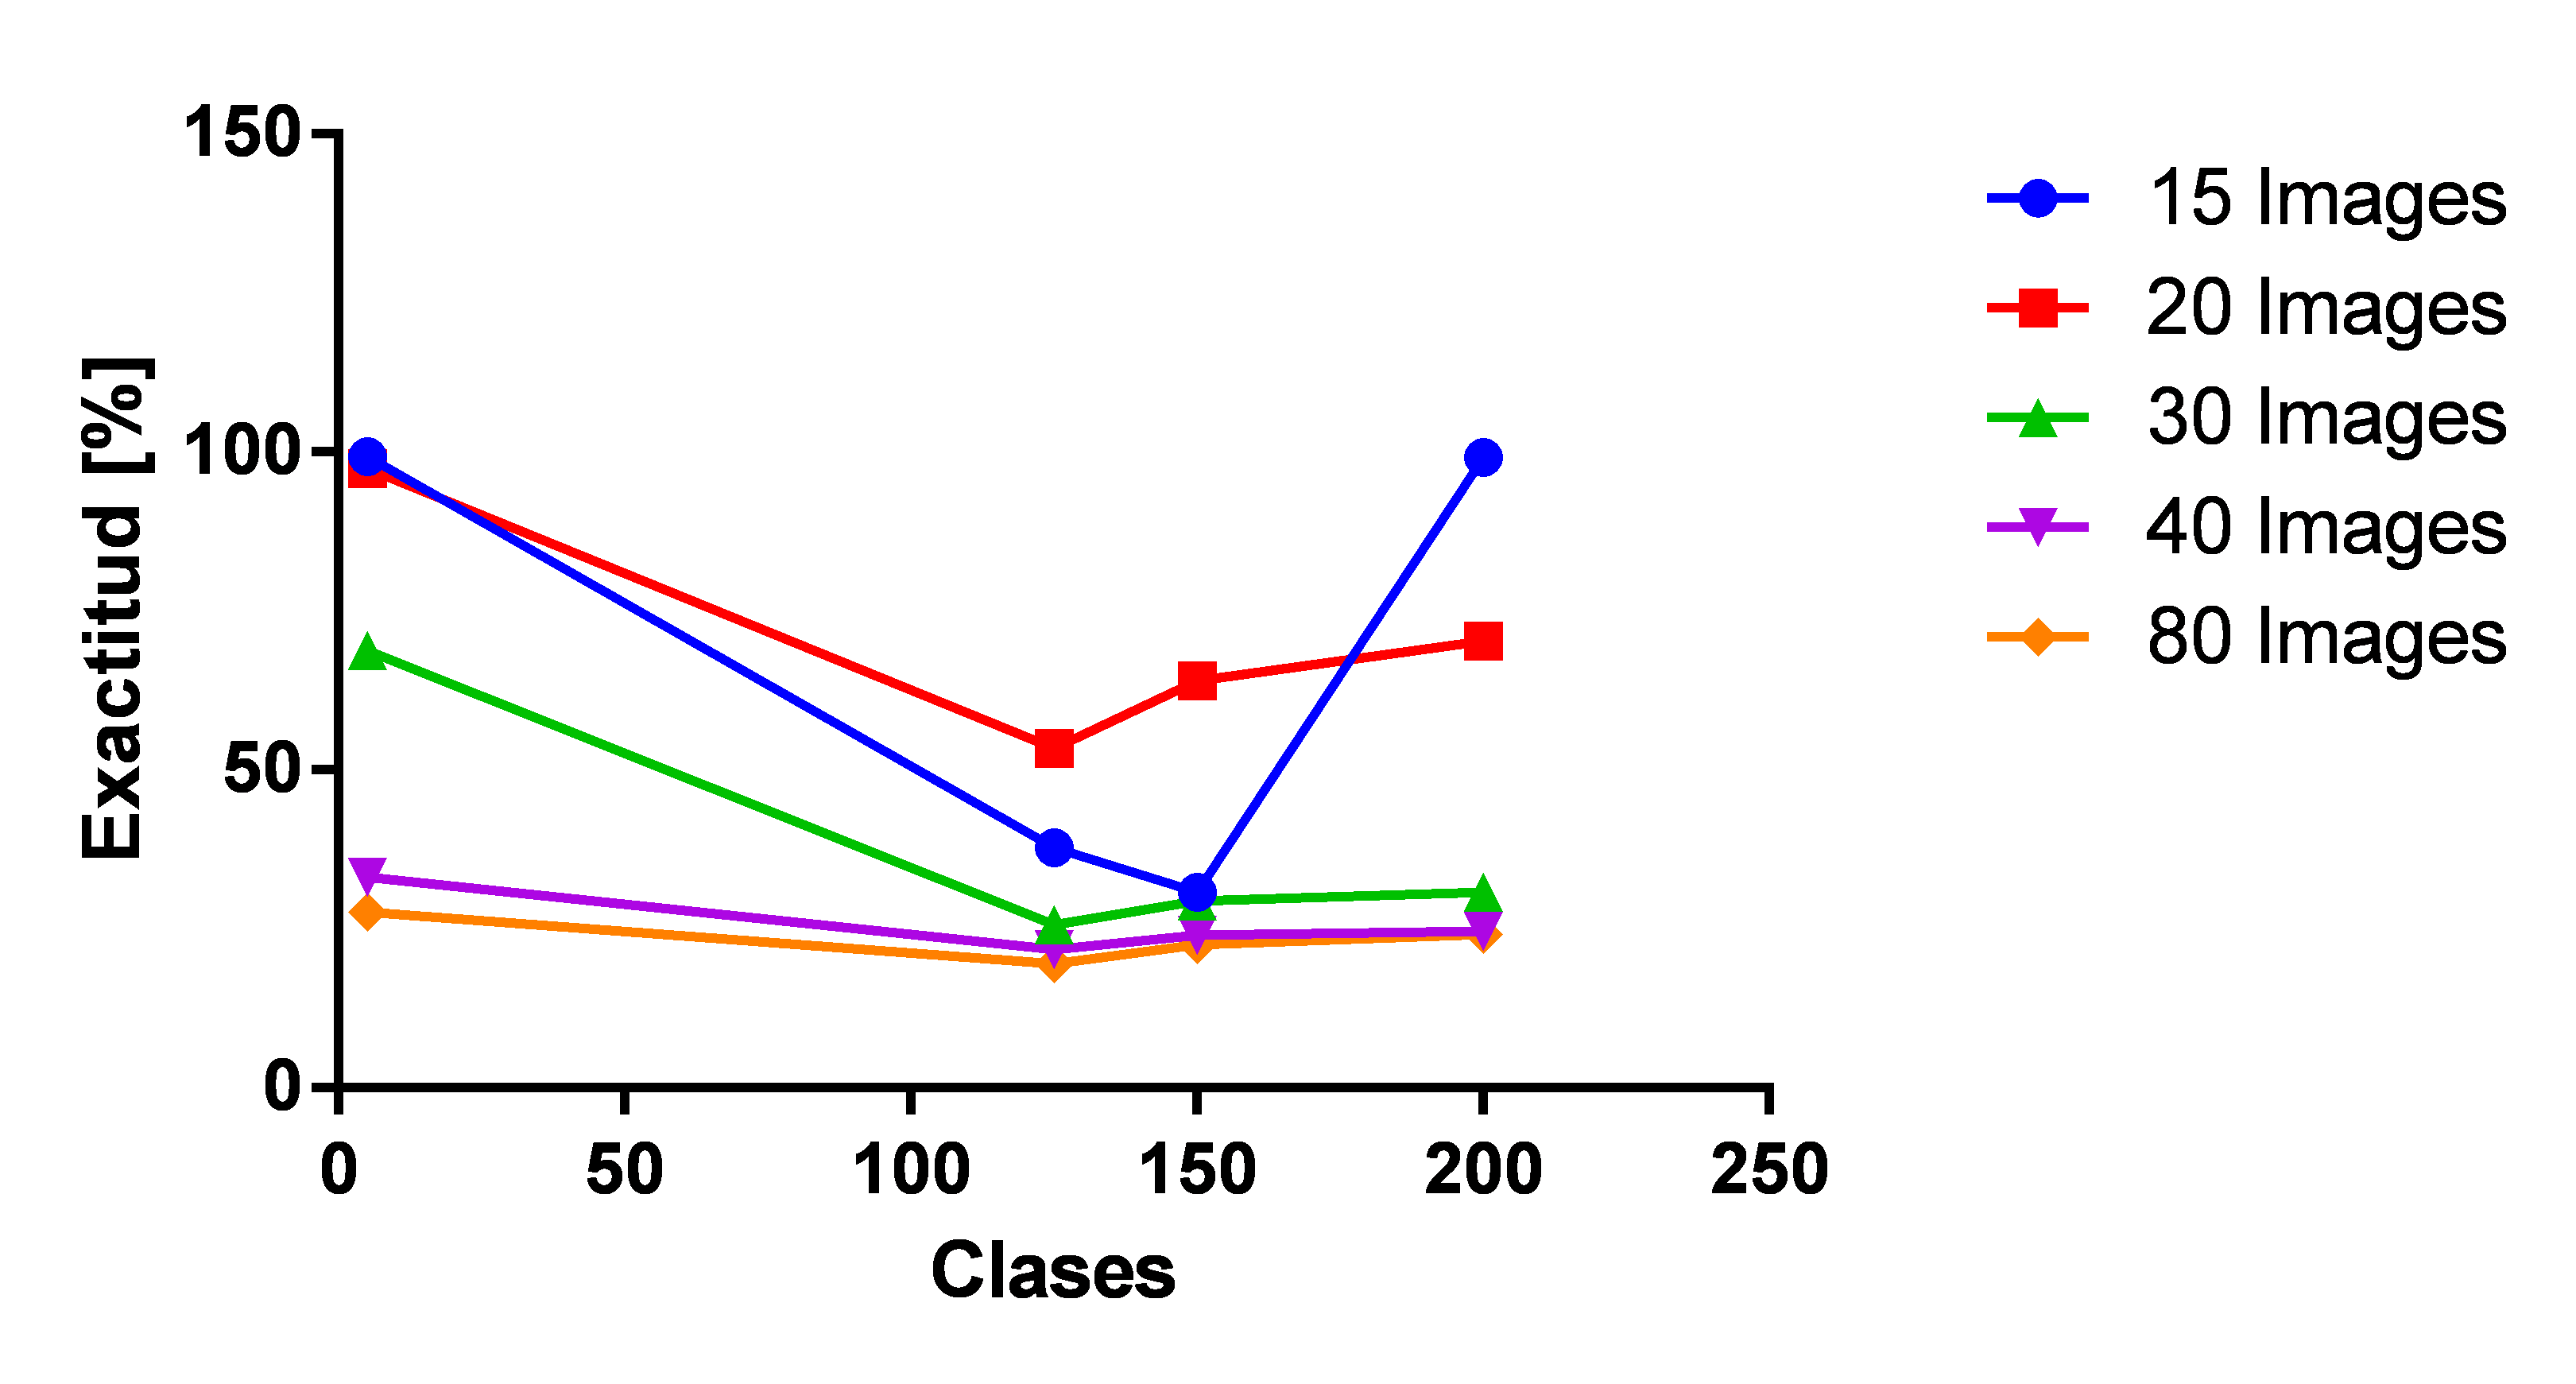
\includegraphics[width=1\linewidth]{clases.png}

\end{figure}

\begin{figure}[ht]
\centering

 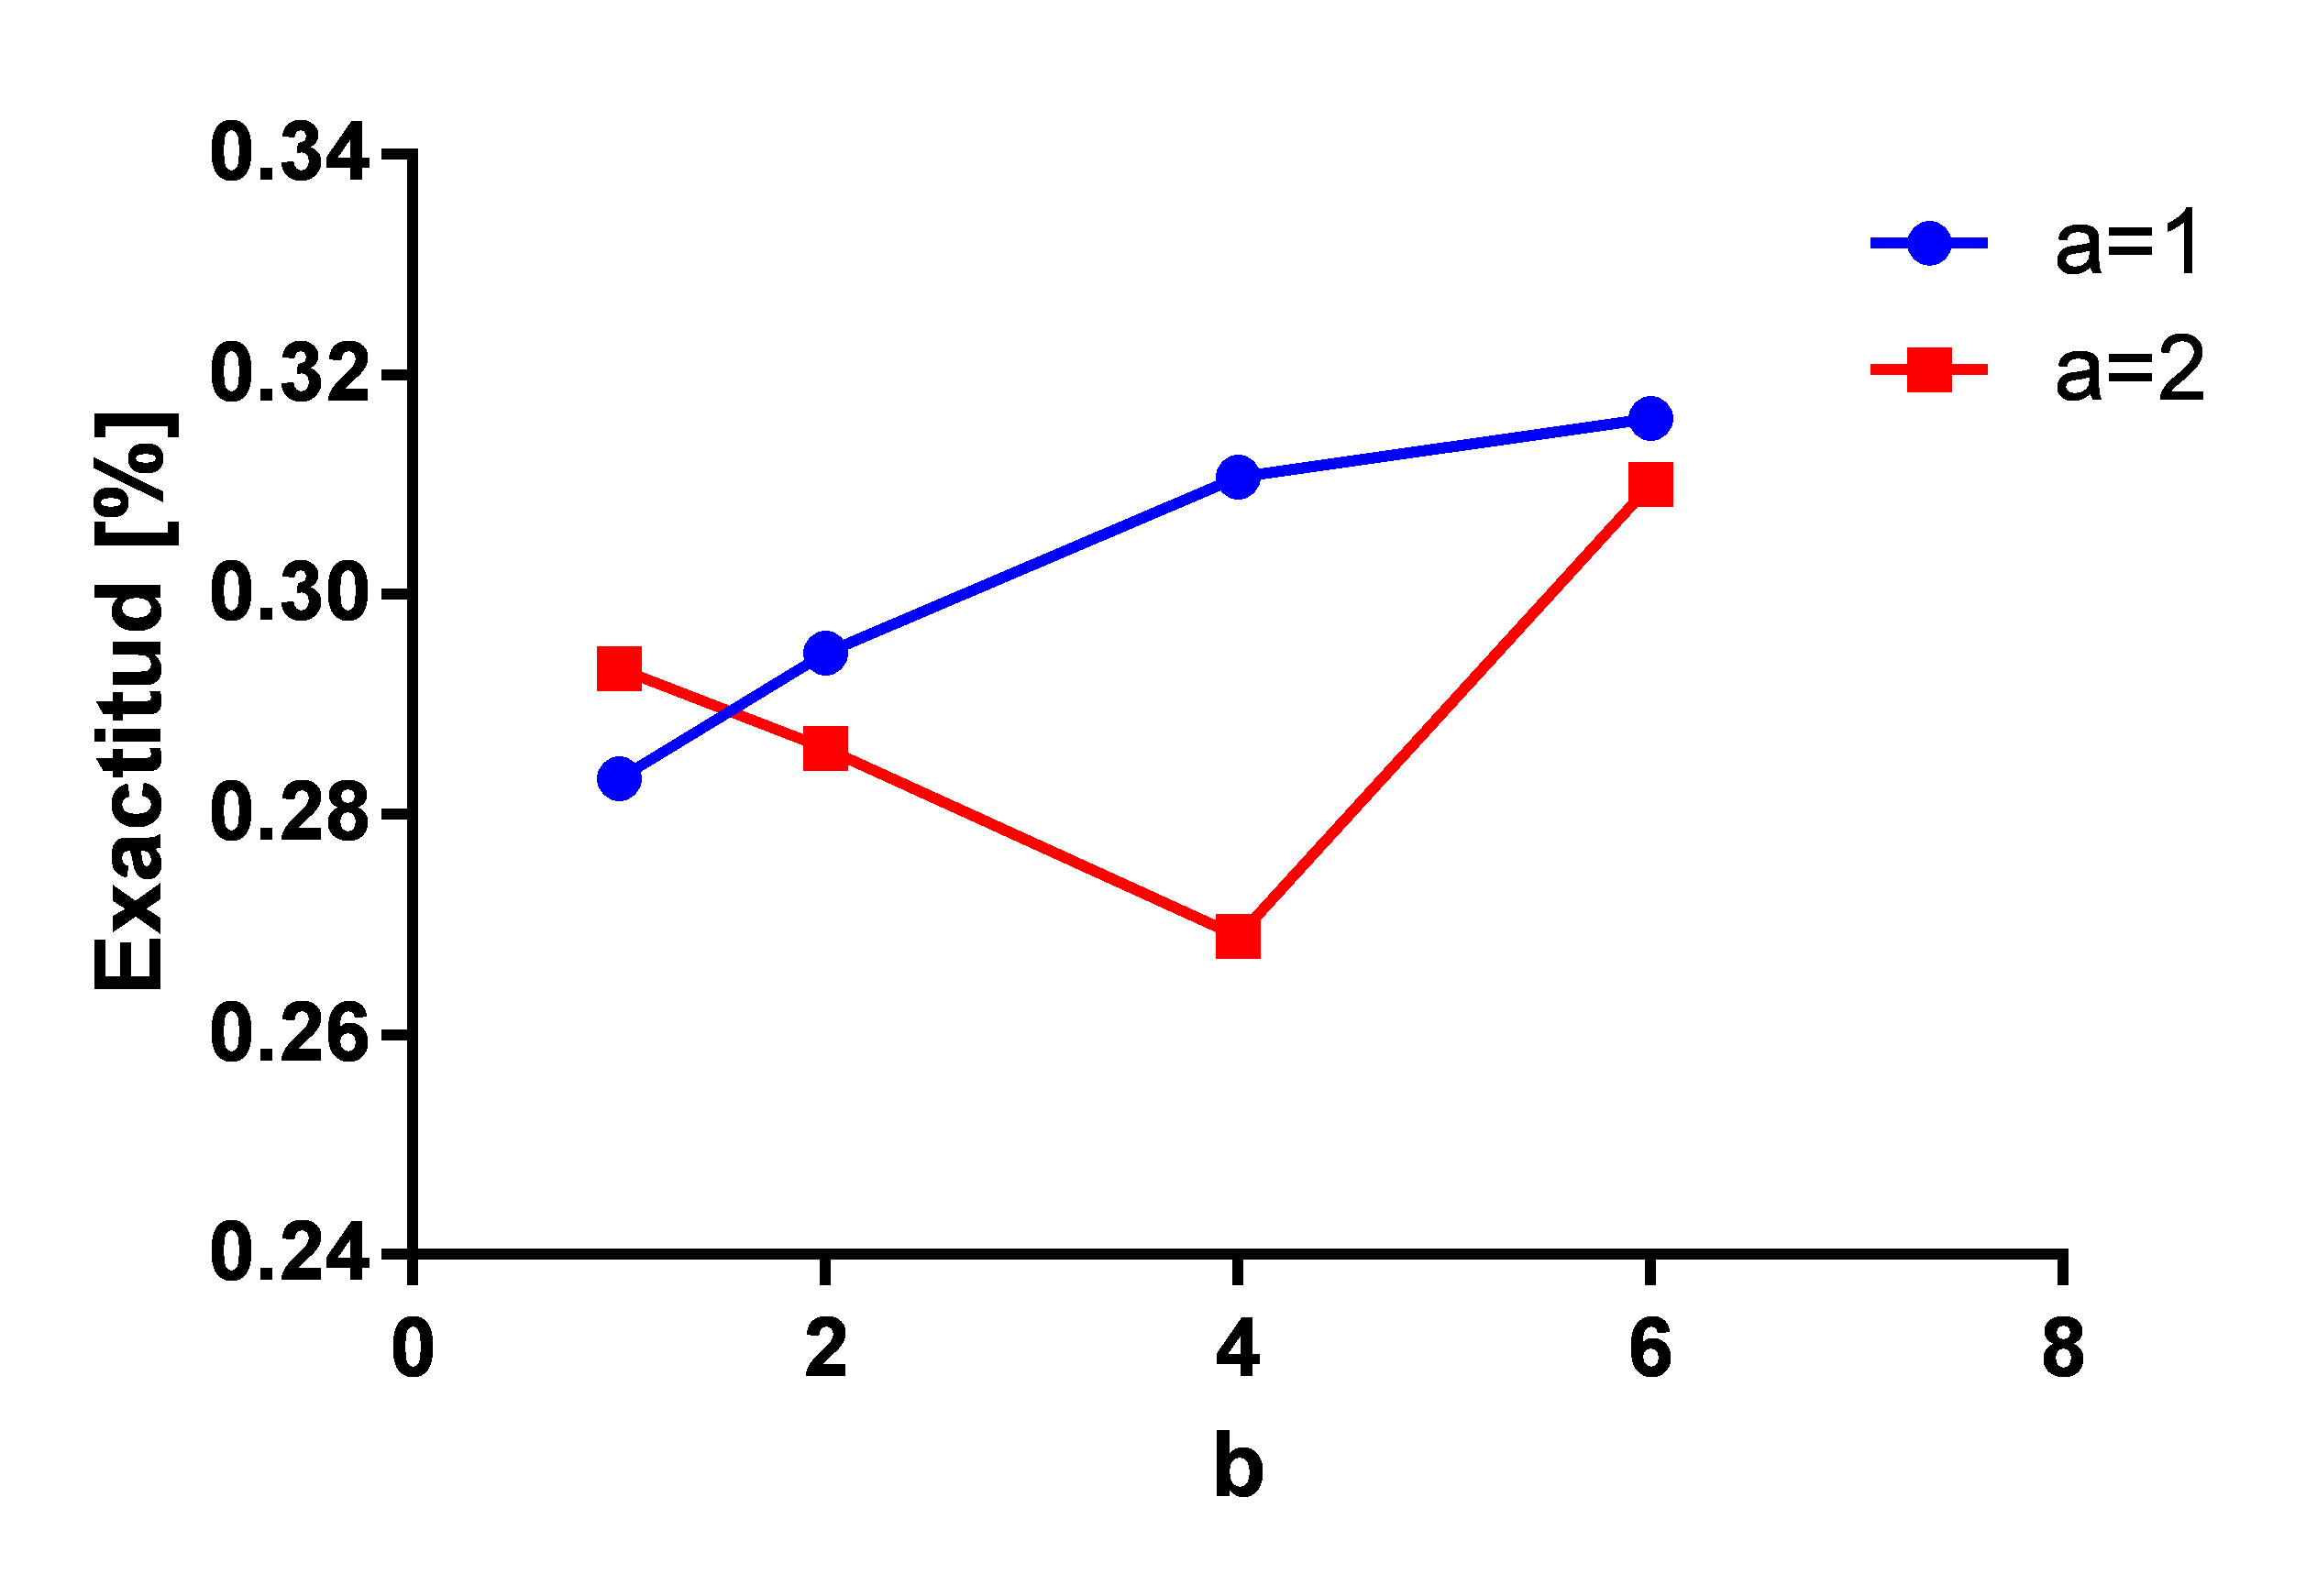
\includegraphics[width=1\linewidth]{Dist_exact.png}

\end{figure}


\subsection{Análisis de resultados}

\begin{figure}[ht]
\centering

 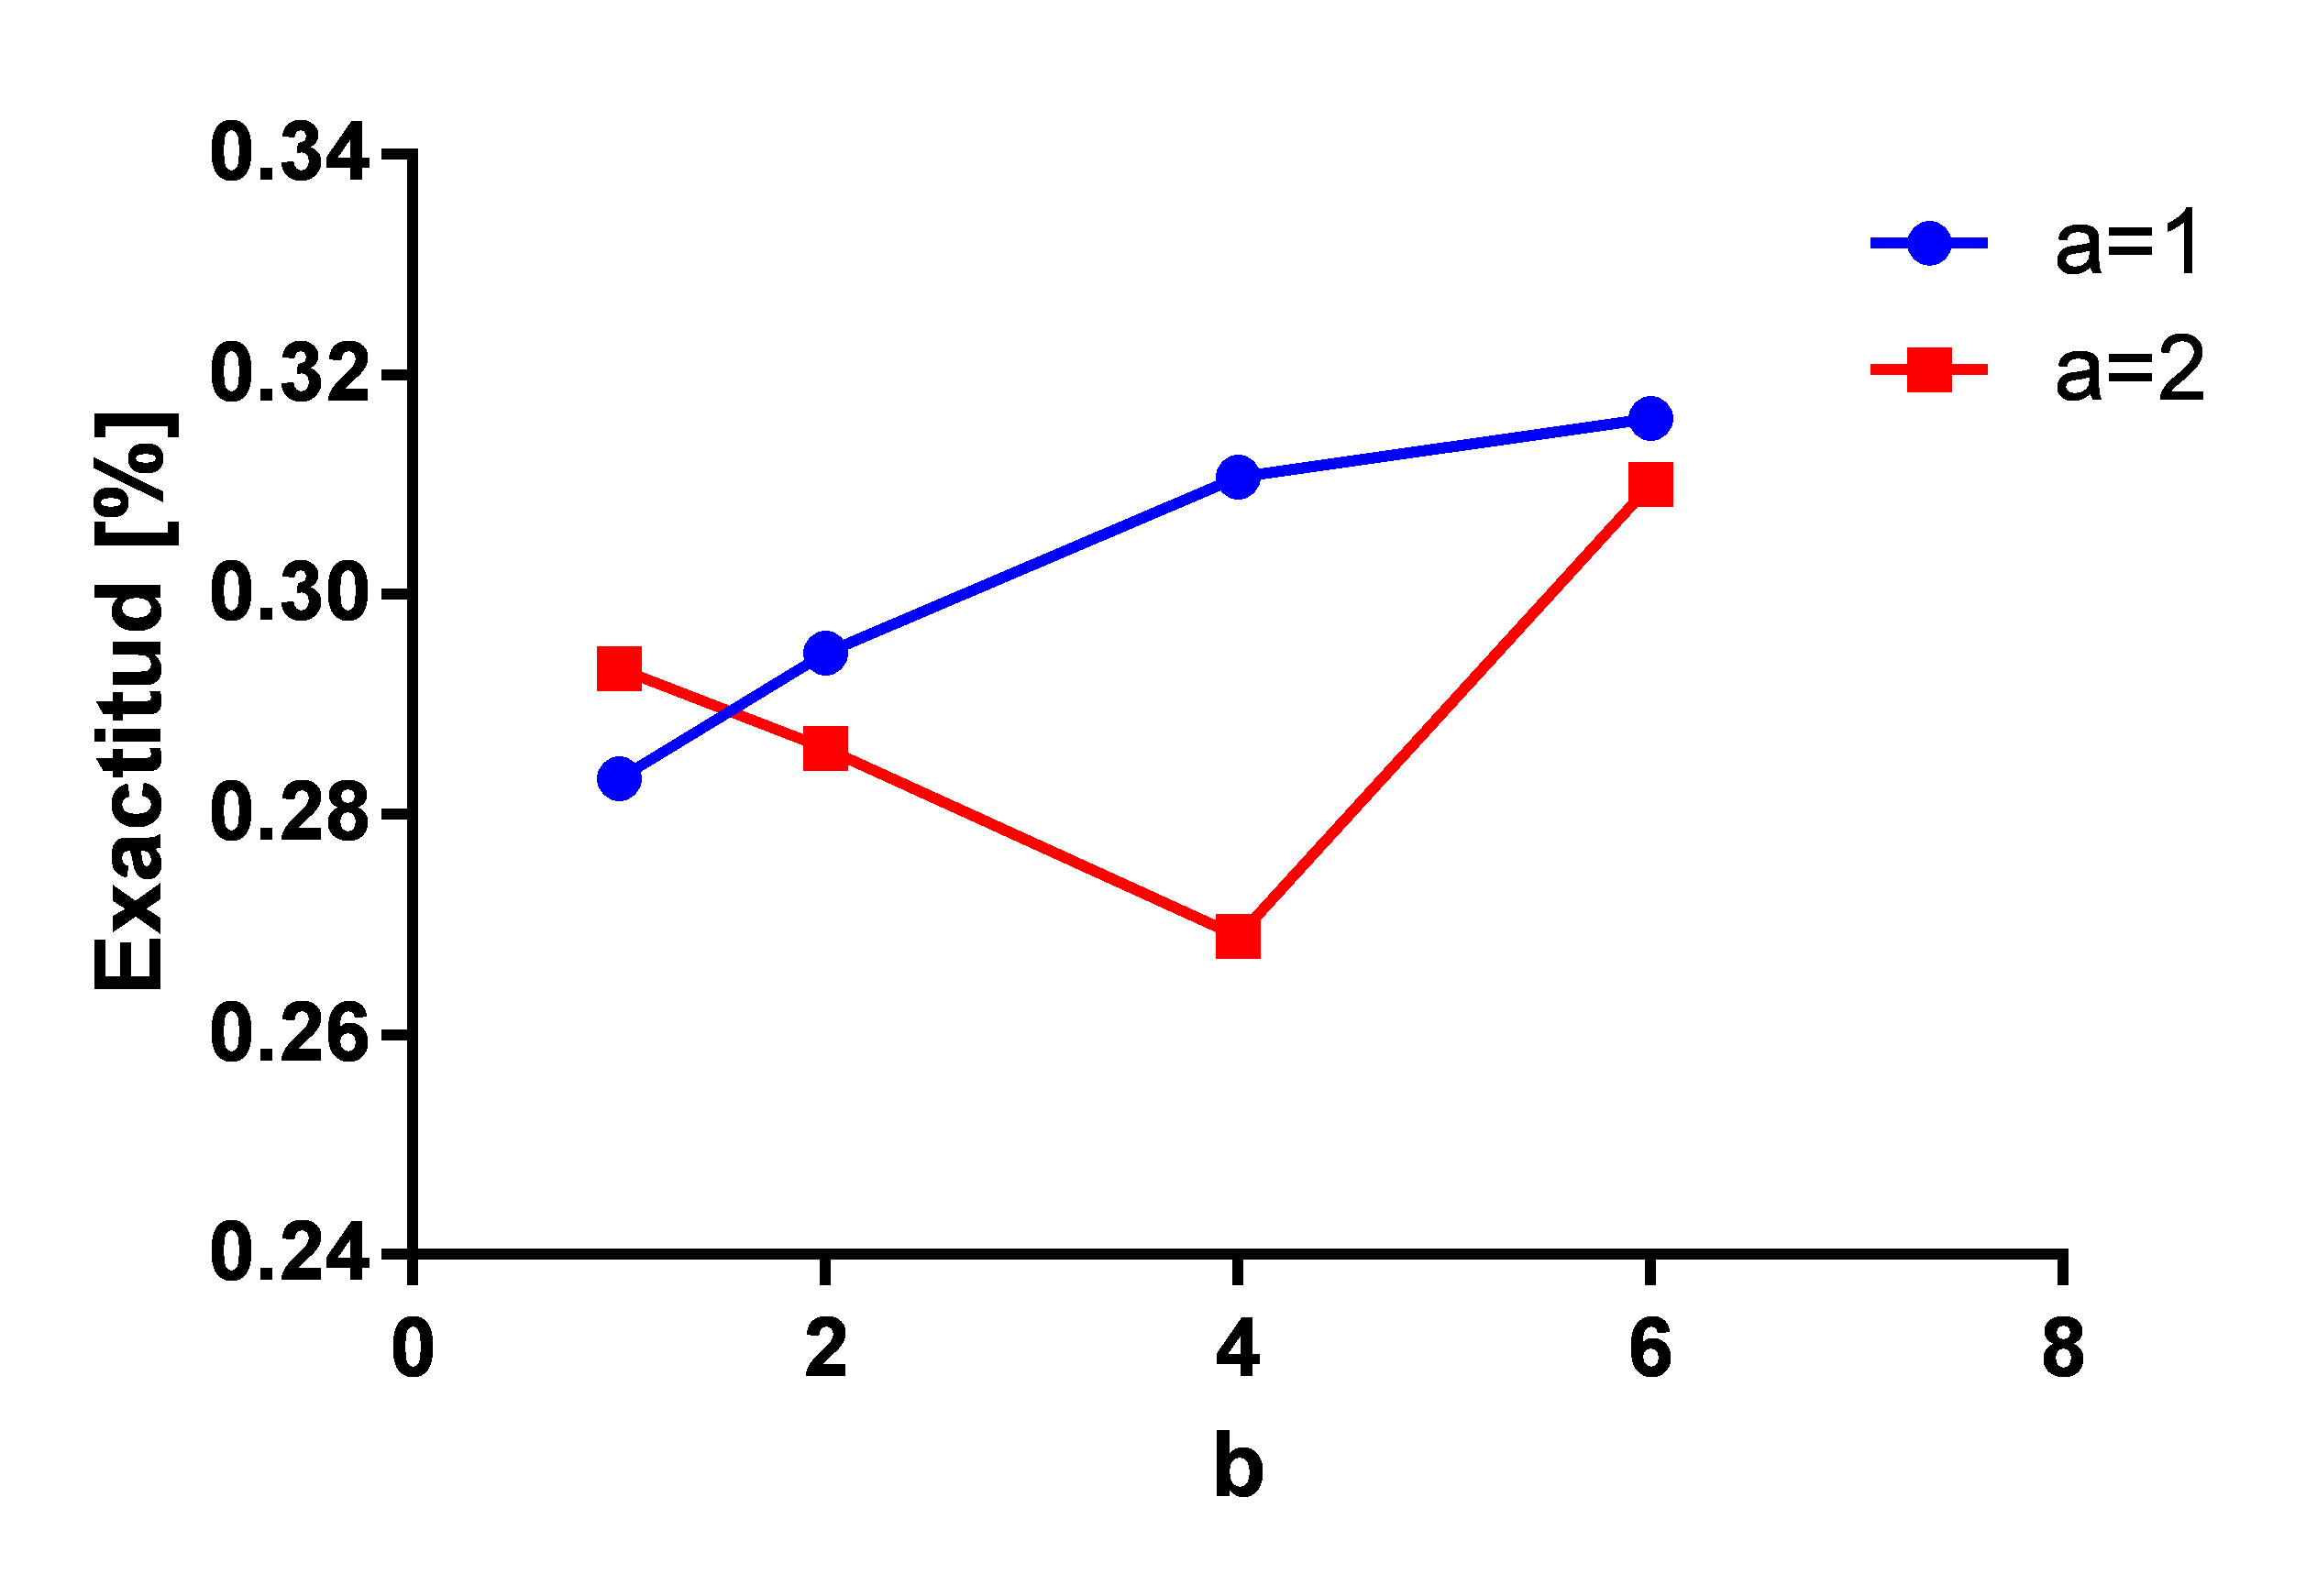
\includegraphics[width=1\linewidth]{Dist_exact.png}

\end{figure}


\begin{figure}[ht]
\centering

 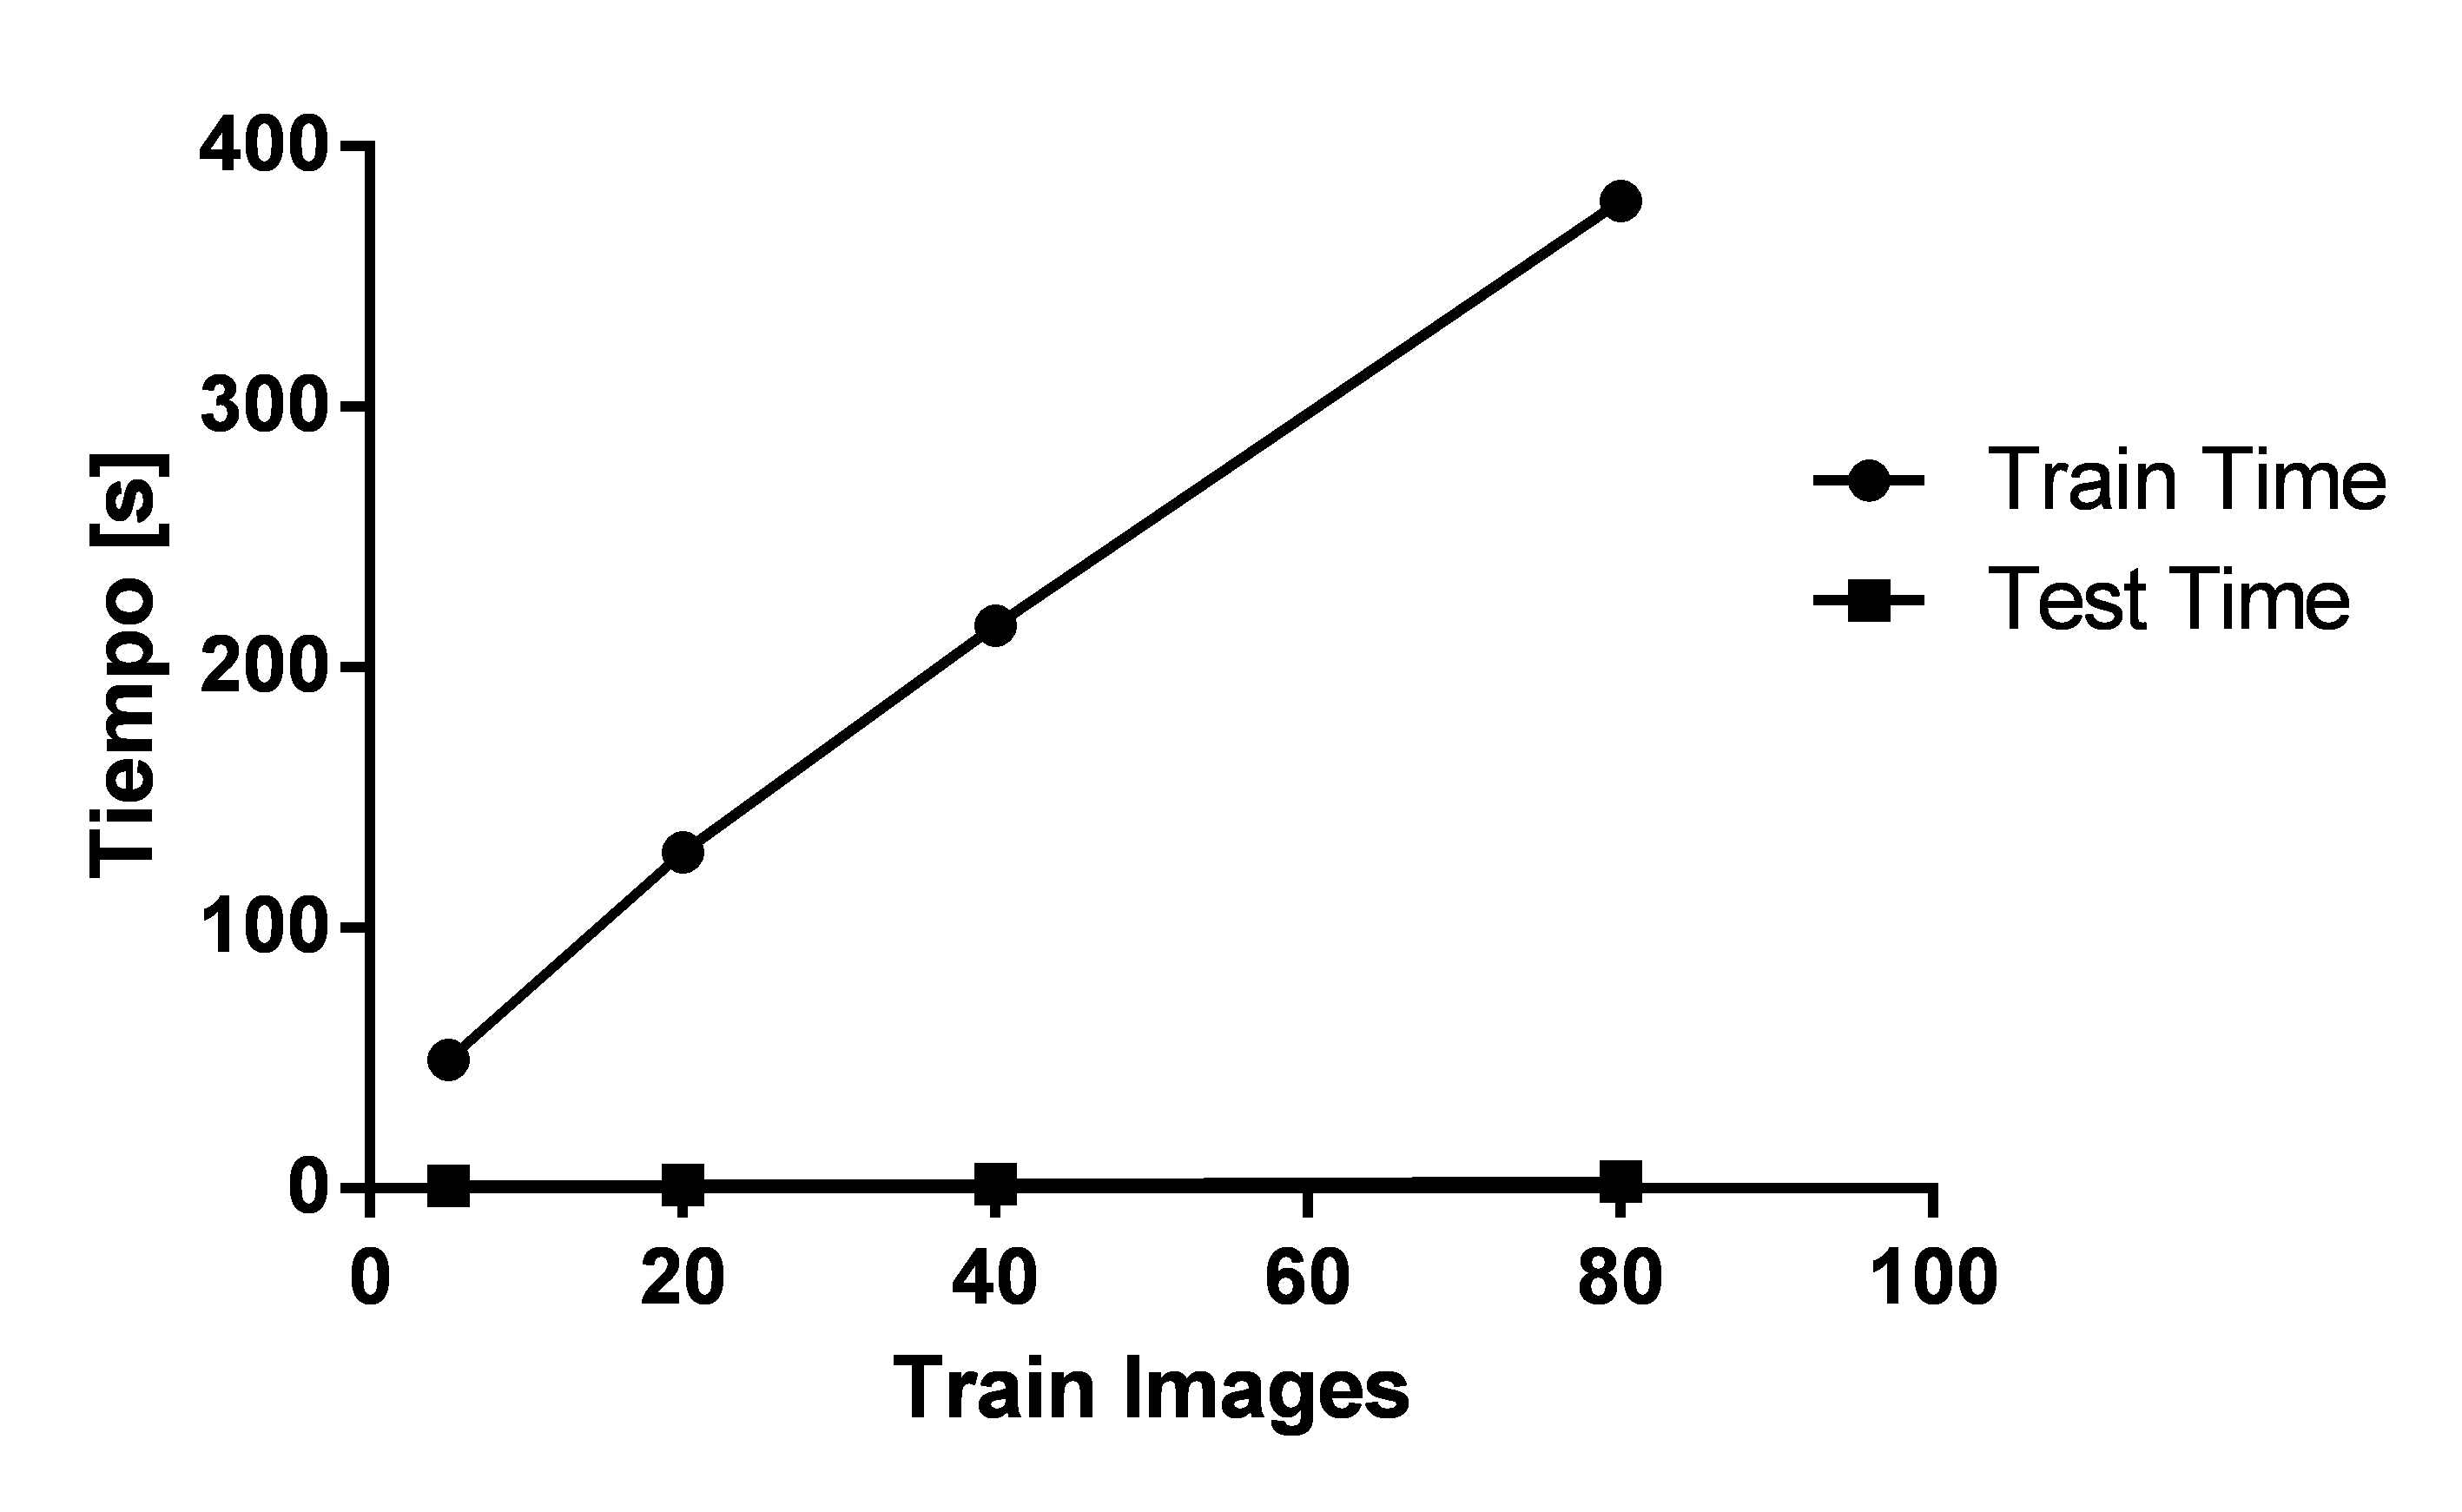
\includegraphics[width=1\linewidth]{Time_train.png}

\end{figure}

\begin{figure}[ht]
\centering

 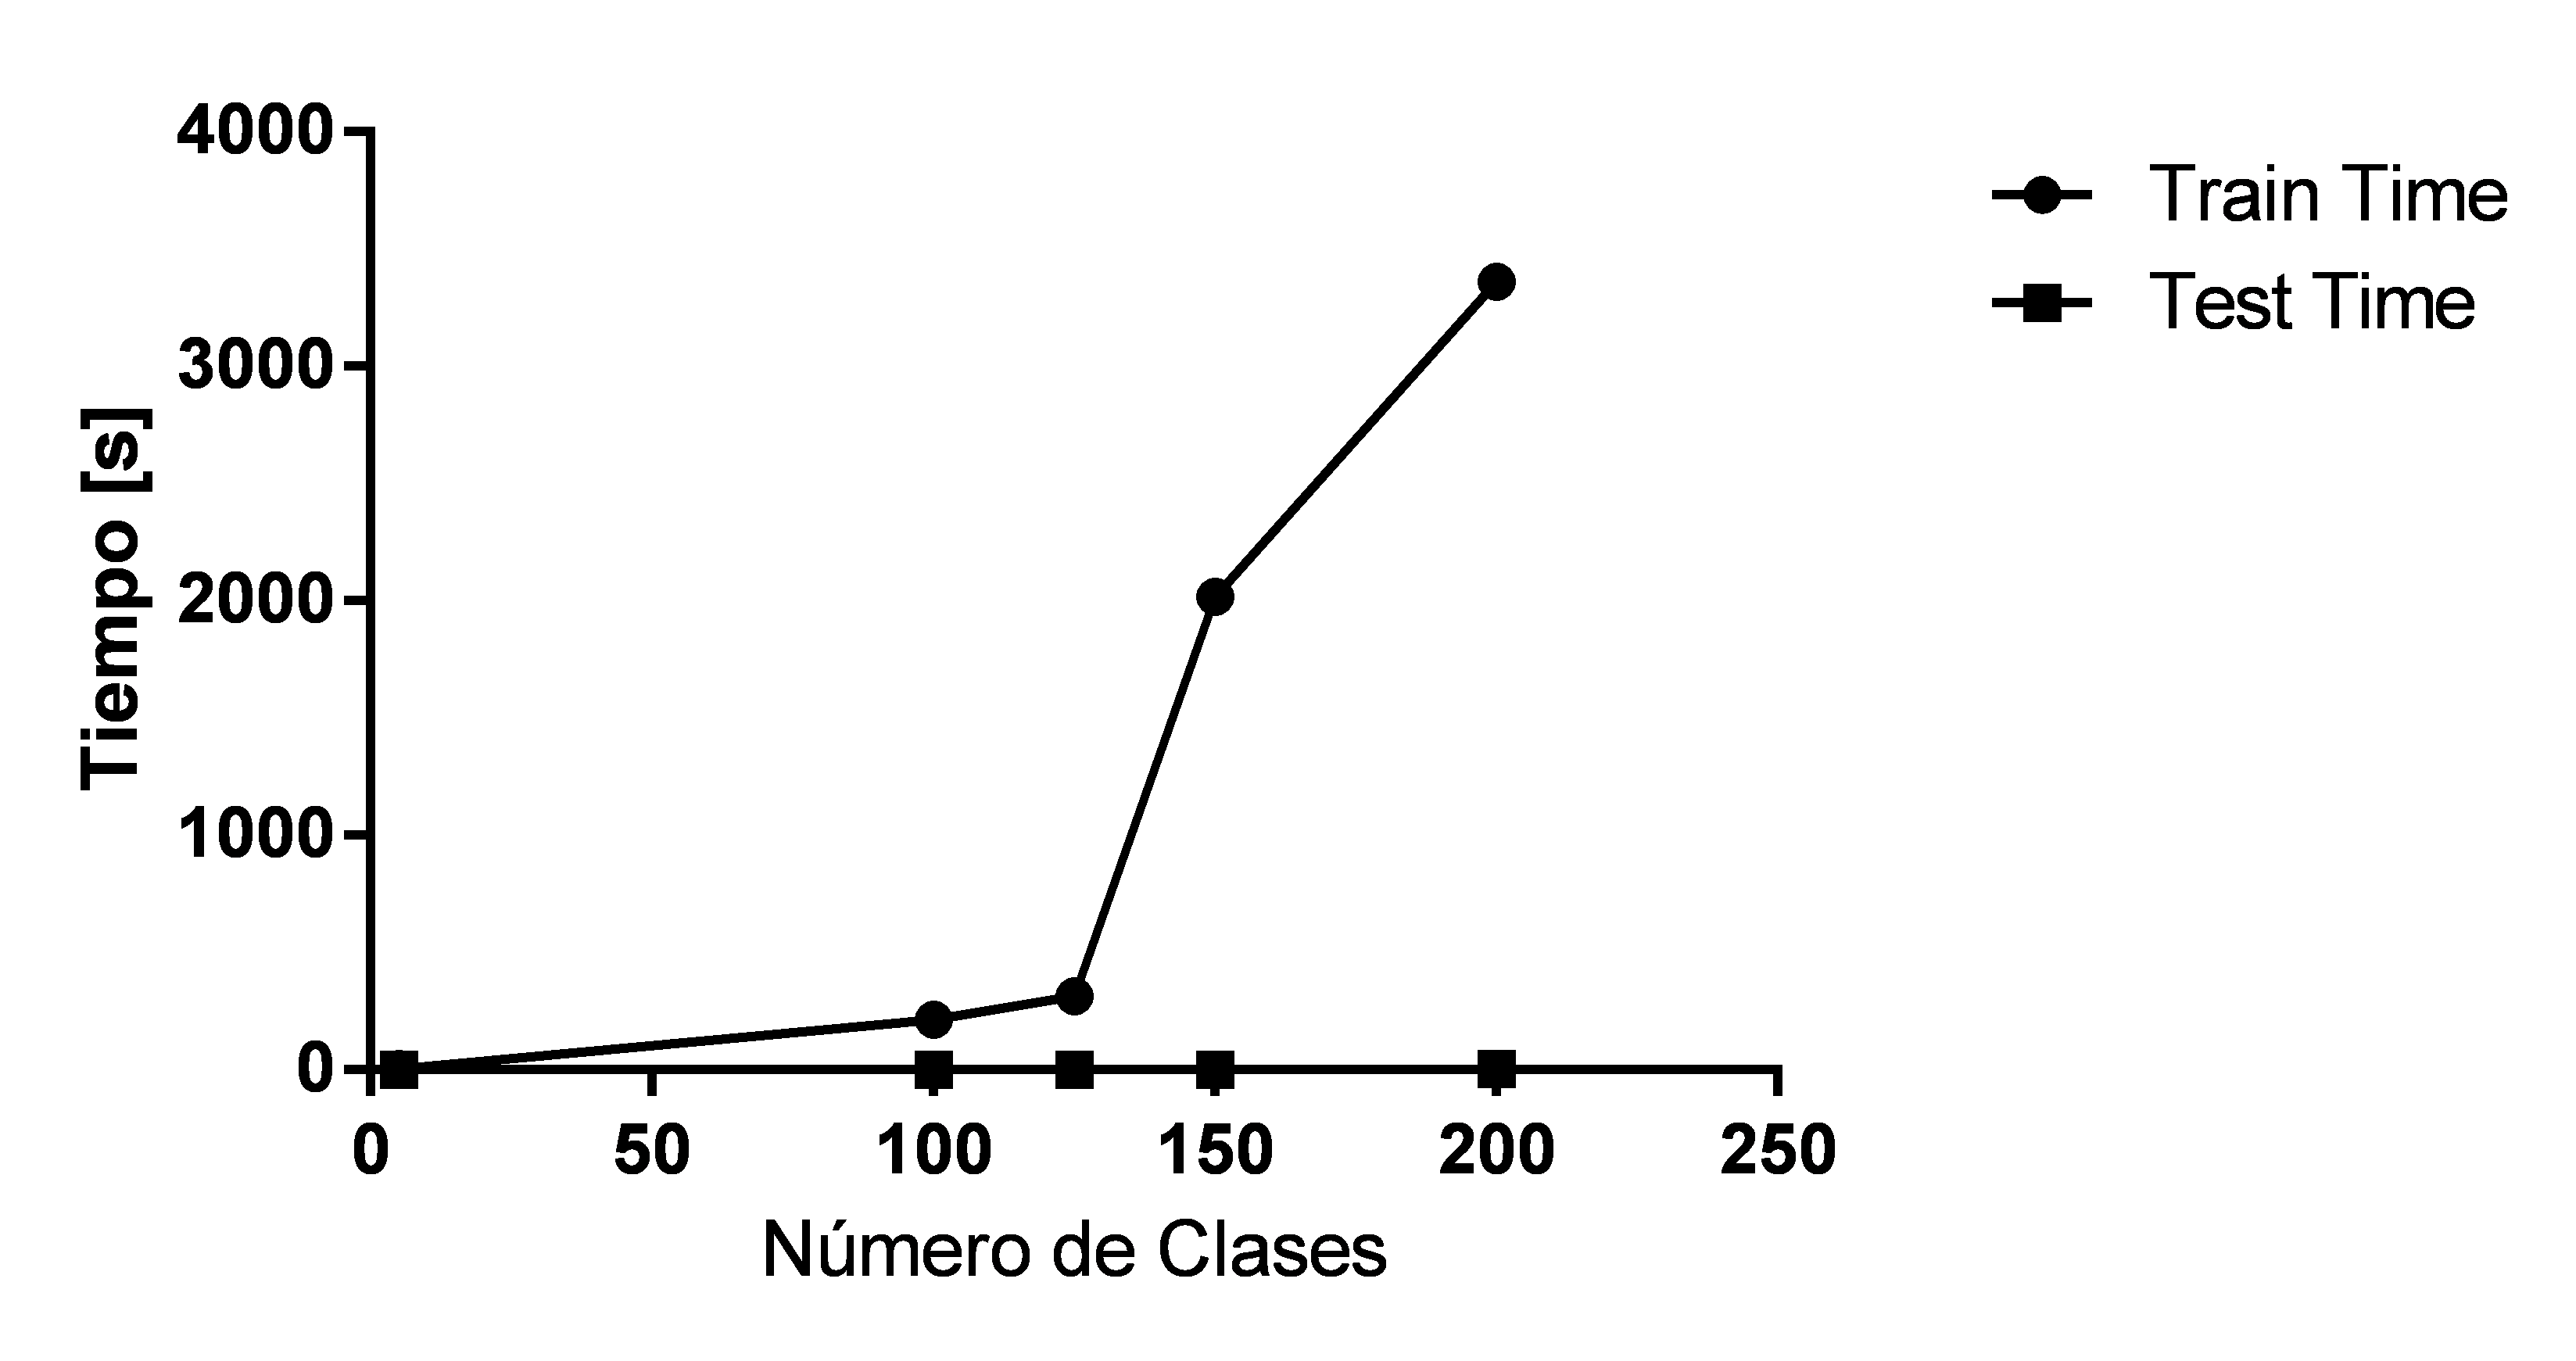
\includegraphics[width=1\linewidth]{Time_clases.png}

\end{figure}

\begin{figure}[ht]
\centering

 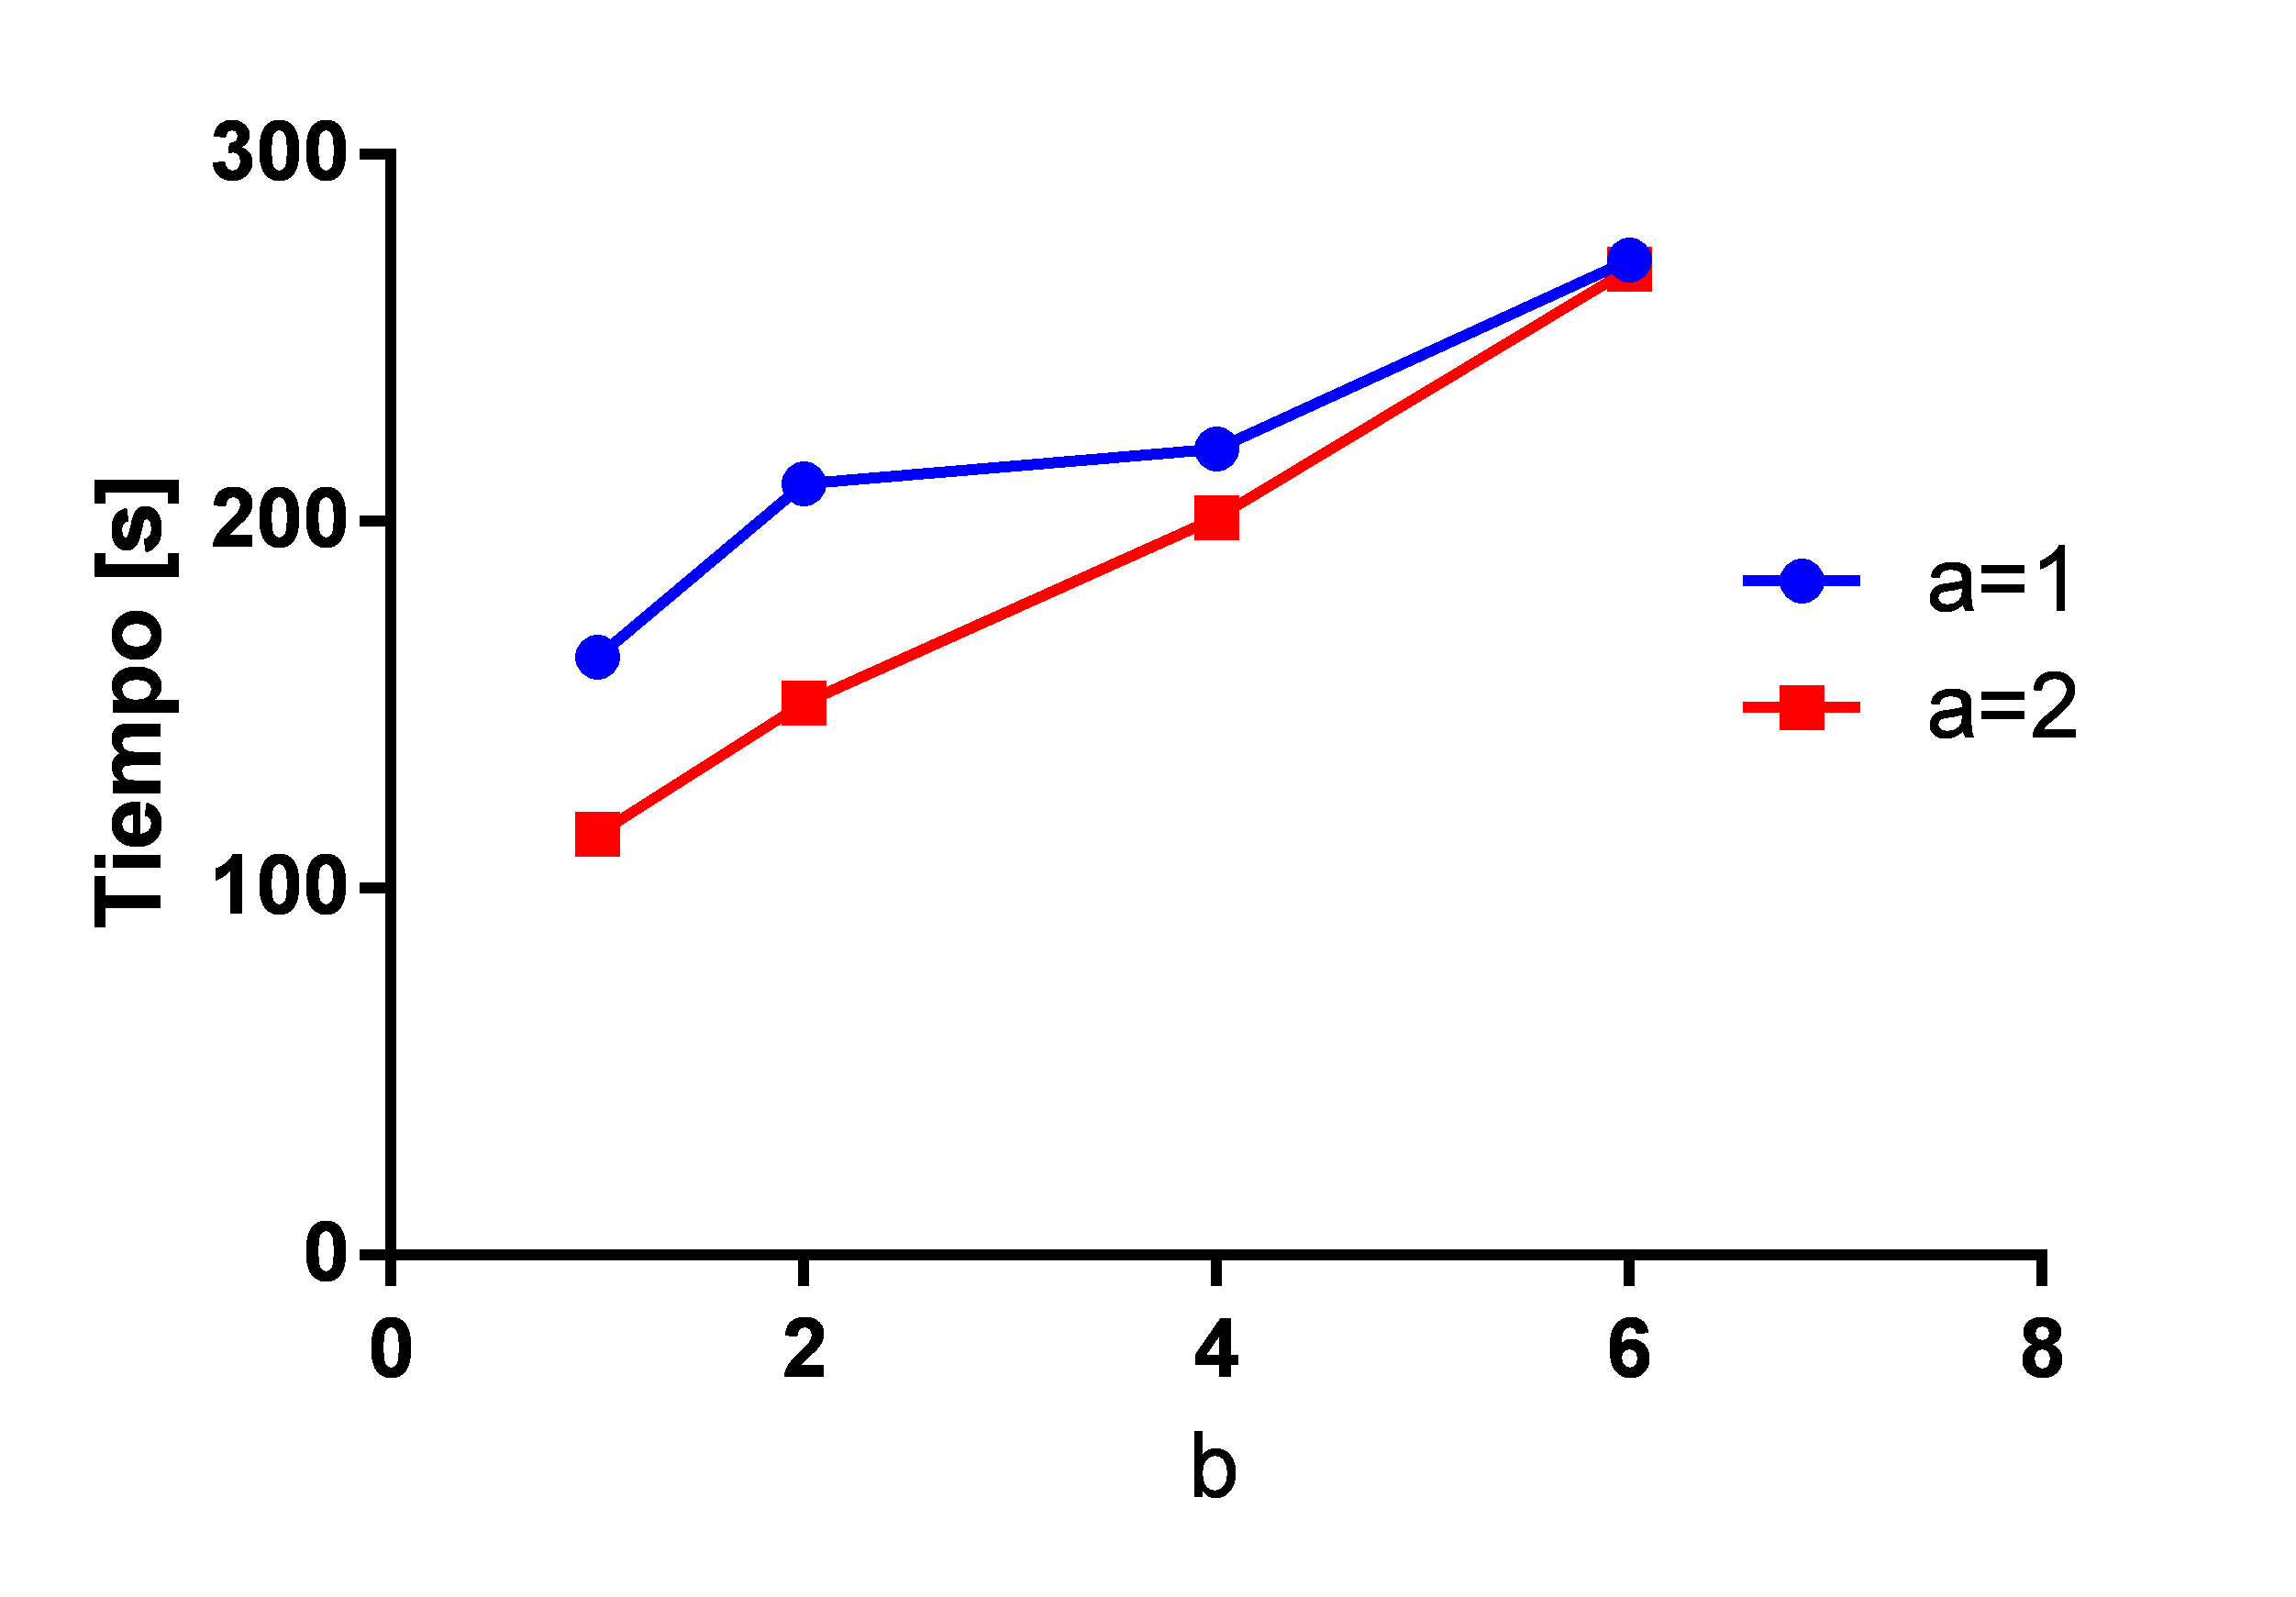
\includegraphics[width=1\linewidth]{Dist_time.png}

\end{figure}

\section{Referencias}

\begin{quote}
   
[1] S. Lazebnik, C. Schmid, and J. Ponce. A Sparse Texture Representation Using Local Affine Regions.\textit{IEEE Transactions on Pattern Analysis and Machine Intelligence} ,  pp. 1265-1278, 2005.
   
   [2] L. Clarkson, "Fast algorithms for the all nearest neighbors problem", \textit{24th IEEE Symp. Foundations of Computer Science}, pp. 226–232, 1983.
   
   [3] B. Schauerte, R. Stiefelhagen, "Learning Robust Color Name Models from Web Images". \textit{In Proceedings of the 21st International Conference on Pattern Recognition (ICPR),}, 2012
    
   [4] Matlab Documentation. TreeBagger class. mathworks.com.
   
\end{quote}

{\small
\bibliographystyle{ieee}
\bibliography{egbib}
}




\end{document}
